\chapter{Computational Challenges prior to Simulating Cooling}

\section{Converting Secular Frequencies to Electric Fields}\label{sec:comp/freqs2aq}

% TODO: Cite more places that solve the Mathieu equation from a geometry of electrodes.
Most solutions of the Mathieu equation in the context of ion trapping start from a certain physical design of electrodes, that (often loosely\cite{AkermanThesis}) is justifying a certain parametrisation for 3 dimensional Mathieu equations. Our only geometry based assumption is that $q_z = 0$, as explained in subsection \ref{ssec:params-trapping}. The following subsections will dive deeper into details of the Mathieu Equation solution, and present a few insights relevant to sympathetic cooling. 

\subsection{Dimensionless Mathieu Equation Solving}

% TODO: Cite literature...
For the sake of completeness, I'll quickly explain how to solve the 1 dimensional Mathieu equation in a numerically practical way. My implemented parametrisation aligns with most parametrisations found in literature:

\begin{equation}
	(a + 2 q \cos(2 \tau)) x = \ddot{x}
	\label{eq:bare-mathieu}
\end{equation}

Where $2\tau \equiv \omega_\mathrm{rf} t$. Substituting a solution of the form:

% TODO: Write this equation
$$x(\tau) = \sum_{-\infty}^\infty $$

Yields the set of equations presented in \ref{eq:gamma_n-relation} between the coefficients $\{\gamma_n\}_{-\infty}^\infty$, with $\beta = 2 \omega_\mathrm{sec}/\omega_\mathrm{rf}$. The main point important to understand, is that we need to find a non-trivial solution, meaning a set $\gamma_n$ coefficients that not all are $0$. The best way to view the equations of all coefficients is via a matrix:

\begin{equation}
% Generated by ChatGPT using the Python code :)
\begin{bmatrix}
\ddots & \ddots & \ddots & & & & \vdots & \vdots & \\
\ddots & -D_{-N} & 1 & 0 & \cdots & 0 & 0 & 0 & \cdots \\
\ddots & 1 & \cdots & \cdots & \cdots & \cdots & \cdots & 0 & \cdots \\
& 0 & \cdots & -D_{-1} & 1 & 0 & \cdots & 0 & \\
& \vdots & \cdots & 1 & -D_0 & 1 & \cdots & \vdots & \\
& 0 & \cdots & 0 & 1 & -D_{1} & \cdots & 0 & \\
\cdots & 0 & \cdots & \cdots & \cdots & \cdots & \cdots & 1 & \ddots \\
\cdots & 0 & 0 & \cdots & 0 & 1 & -D_{N} & \ddots & \ddots \\
& \vdots & \vdots & & & \ddots & \ddots & \ddots & \ddots \\
\end{bmatrix}
\begin{bmatrix}
\vdots \\
\gamma_{-N} \\
\vdots \\
\gamma_{-1} \\
\gamma_0 \\
\gamma_{1} \\
\vdots \\
\gamma_{N} \\
\vdots
\end{bmatrix}
\overset{!}{=}
\begin{bmatrix}
\vdots \\
0 \\
\vdots \\
0 \\
0 \\
0 \\
\vdots \\
0 \\
\vdots
\end{bmatrix}
\end{equation}

Where similarly to \ref{eq:gamma_n-relation}:

$$D_n = \frac{a - \left(\beta + n\right)^2}{q}$$

One can easily see that $D_n$ increases $\sim n^2$, which promises the target $\beta$ solution might converge if a finite matrix will be used. To require a non-trivial solution, we simply require the matrix to have a $0$ determinant, thus supplying us an equation for $\beta$ that can be solved easily numerically, for matrix size $2N+1$. Inserting the $\beta$ into the matrix, and inspecting the kernel of it, will give us the $\gamma_n$ coefficients of the solution, and we'd be able to easily verify they indeed decrease with $|n|$, and are that $\gamma_0$ is the most dominant.

The verification of this solution was implemented in a Matplotlib\cite{Matplotlib} based interactive plot, presented in figures \ref{fig:pure-mathieu-coefficients} \& \ref{fig:pure-mathieu-fft}.

\begin{figure}
	\begin{center}
		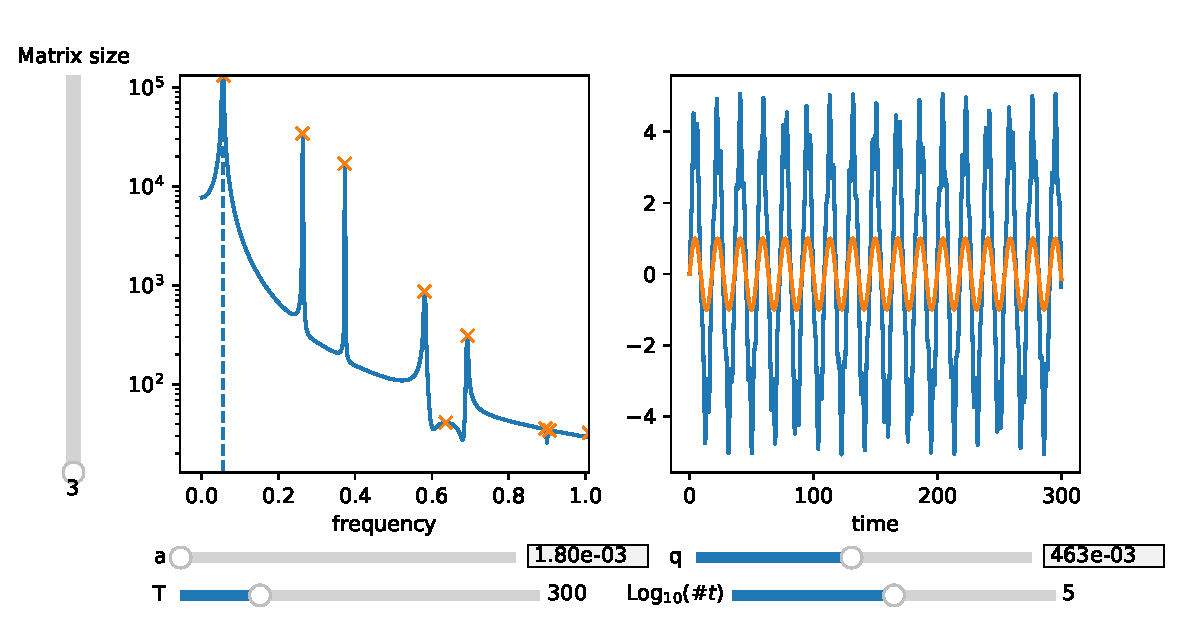
\includegraphics[width=0.95\textwidth]{graphics/pure-mathieu-fft.pdf}
	\end{center}
	\caption{Matplotlib interactive plot presenting the 1 dimensional solution of the Mathieu equation, with a spectrum analysis demonstrating the correct matrix based solution of $\beta$ in the dashed line. The orange sinusoidal line in the right axes is a simple cosine line with the right phase and the calculated $\beta$ as a frequency. The $T$ and $\mathrm{Log}_{10}(\#t)$ sliders control the total time duration of the numerical ODE solution and the time spacing finesse, respectively.}
	\label{fig:pure-mathieu-fft}
\end{figure}

\begin{figure}
	\begin{center}
		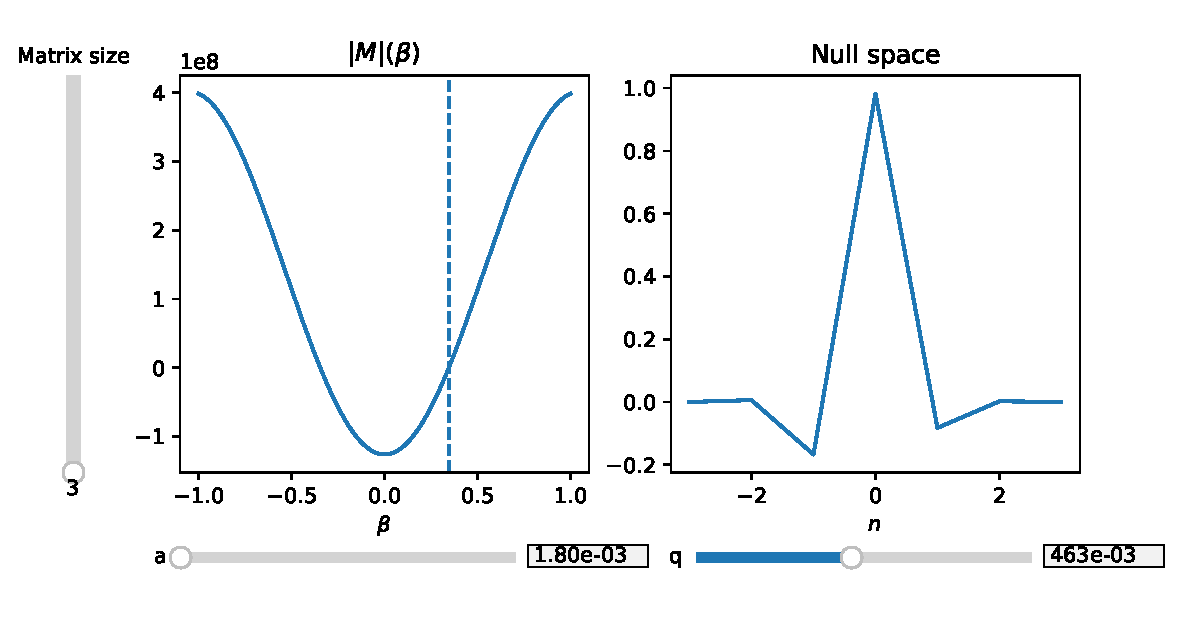
\includegraphics[width=0.95\textwidth]{graphics/pure-mathieu-kernel.pdf}
	\end{center}
	\caption{Matplotlib interactive plot demonstrating the fast decay of the Mathieu equation's solution's $\gamma_n$ (normalized) coefficients, as $|n|$ increases. The dashed $\beta$ line represents the $\beta$ which zeros the matrix determinant.}
	\label{fig:pure-mathieu-coefficients}
\end{figure}

Interactive plot \ref{fig:pure-mathieu-fft} can be also useful for inspecting the roughness of the motion as a function of $a$ and $q$. As expected, a high $q$ and a lower $a$ produce more 'RF-noisy' motion near the peaks of the oscillatory, secular motion. Also, satisfyingly, there's barely any difference in the $\beta$ accuracy as $N$ is increased, even when starting from $N=3$. Hence, this parameter was practically hard-coded in all the simulations etc. to $N=7$.

% TODO: Cite this
Most Mathieu stability diagrams found in literature, assume that geometry dictates $a_x = a_y$, and like us, that $q_z = 0$. Thanks to equation \ref{eq:laplace}, this suggests that one can plot a single Mathieu stability diagram for a 3 dimensional trap using a single Mathieu stability diagram for $(a_r,q_r)$ where $a_r \equiv a_x = a_y = -a_z/2$ and $q_r = q_x = -q_y$ as axes. I find these stability diagrams confusing, as they need to also take care of correctly mirroring $q_x = -q_y$ to satisfy stability in both $x$ \& $y$ spatial dimensions (where the $z$ axis is trivially stable). Figure \ref{fig:mathieu-stability} presents a much simpler alternative to show the stability of a 3 dimensional trap, without even imposing cylindrical symmetry which shouldn't be physically unimplementable.

\begin{figure}
	\begin{center}
		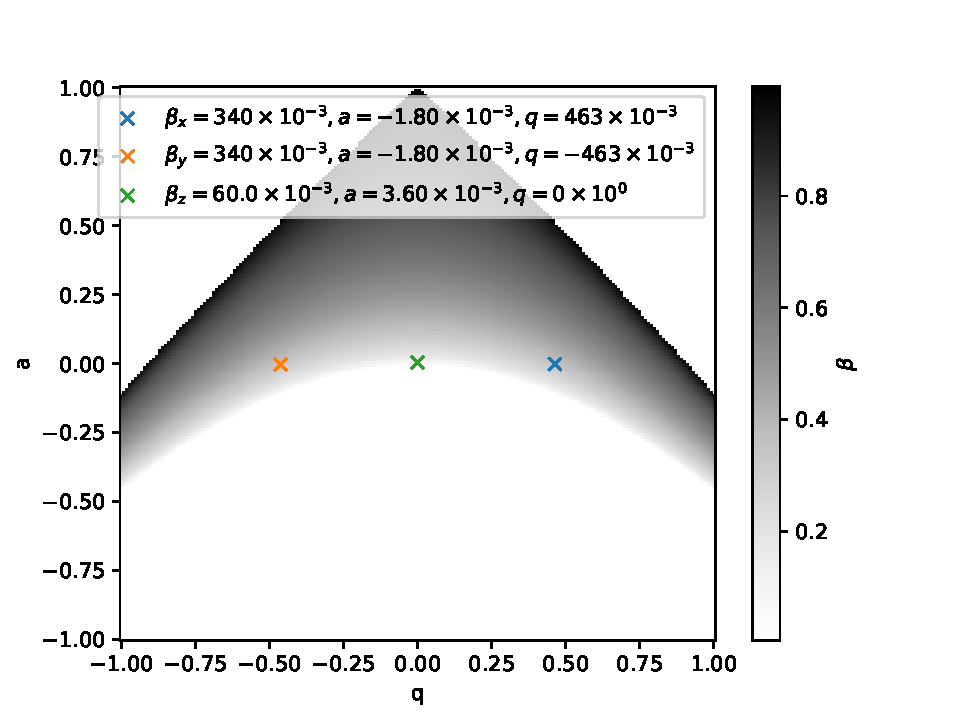
\includegraphics[width=0.86\textwidth]{graphics/pure-mathieu-stability.pdf}
	\end{center}
	\caption{Mathieu Stability diagram, with shades of gray marking the magnitude of $\beta$. The $\times$ signs are specific $\beta$ values, that were used in many simulations of this work - $\beta$s corresponding to secular frequencies $(8.5, 8.5, 1.5)\mathrm{kHz}$, with $f_\mathrm{rf} = 50\mathrm{kHz}$.}
	\label{fig:mathieu-stability}
\end{figure}

\subsection{A Non-Trivial Secular Frequency Mass Dependence}\label{ssec:non-trivial-mass-dep}

In my literature I have seen no authors discuss the secular frequency related implications encountered when 2 different masses are trapped in the same Ion trap. This detail is naturally of interest to us as we are interested in sympathetic cooling. Let's discuss this question in 1 spatial dimension: Given a $(a,q)$ pair producing a dimensionless secular frequency $\beta_0$ for mass $m_{cooler}$, what would be the secular frequency experienced by a mass $m_{target}$ experiencing the same forces? In a pure harmonic oscillator, the same $k = m_{cooler} \omega_{\mathrm{sec(cooler)}}^2 = m_{cooler} (\beta_0 \omega_\mathrm{rf}/2)^2$ is applied to any mass, and we get a secular frequency for $m_{target}$ of:

\begin{equation}
	\omega_\mathrm{sec(target)} = \omega_\mathrm{sec(cooler)}\sqrt{\frac{m_{cooler}}{m_{target}}} 
	\label{eq:mathieu-naive-sec-freq}
\end{equation}

Is that true in a Mathieu trap? The process of generating a dimensionless $(a,q)$ from the original equation of motion (equation \ref{eq:mathieu-source}) involves dividing the equation by the mass, meaning that $(a,q)\propto 1/m_{cooler}$. Hence the real secular frequency of $m_{target}$ can be obtained by calculating $\beta_{target}$ given the pair:

$$(a,q)\cdot \frac{m_{cooler}}{m_{target}}$$

The dependence of $\beta_{target}$ as a function of the mass ratio is depicted in figure \ref{fig:mathieu-mass-dep}. This insight invites defining 2 decoupled, boolean parameters for the simulation, named \texttt{micromotion} \& \texttt{naive\_freqs}. Table \ref{tbl:naive_freqs-micromotion} is a truth table explaining what trapping forces are applied in each combination of these parameters. A separate definition of these parameters is laid out afterwards for completeness.
% TODO: Make sure this 'afterwards' is correct - depends upon the final state of the document

\begin{figure}
	\begin{center}
		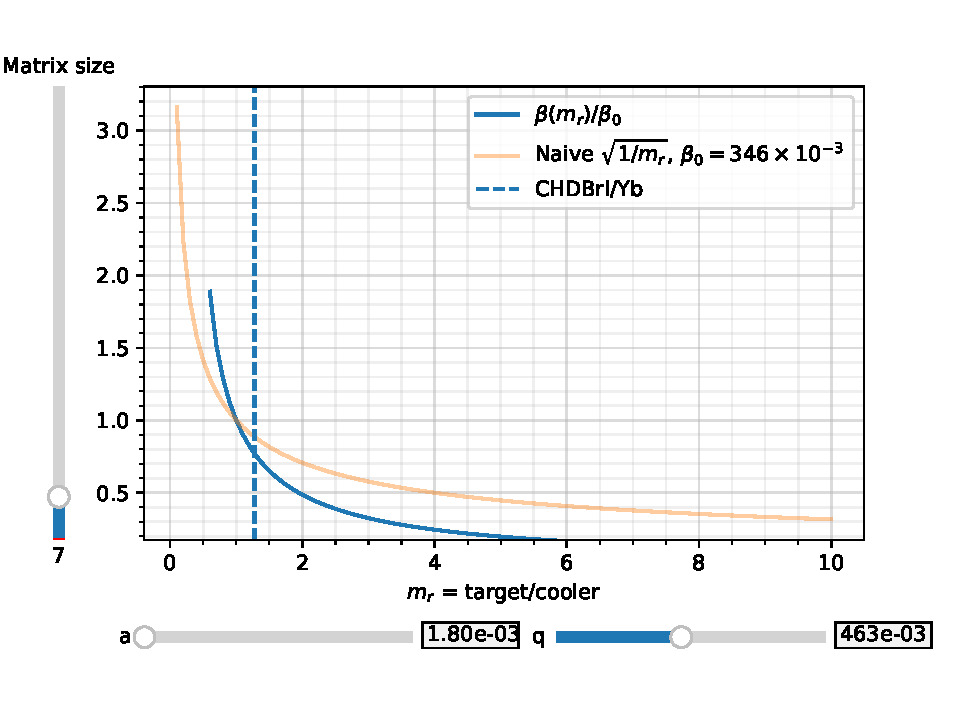
\includegraphics[width=0.86\textwidth]{graphics/mathieu-mass-dep.pdf}
	\end{center}
	\caption{A Matplotlib interactive plot showing the non-trivial dependence of the secular frequencies of a 'target' mass (represented in blue), given a Mathieu trap with $(a,q)$ that define a certain secular frequency for a 'cooler' mass, termed $\beta_0$. The $(a,q)$ values used here, implement the $x$-axis Mathieu force that was used in the simulations that produced the summarized results in figure \ref{fig:LAMMPS_summarized_naive_freqs-micromotion}, which also shows the possible secular frequencies' absolute values in $\mathrm{kHz}$.}
	\label{fig:mathieu-mass-dep}
\end{figure}

\begin{table}[h]
\centering
\begin{tabularx}{\textwidth}{cccX}
\toprule
\texttt{mm} & $\sqrt{m_r}$ & \textbf{Physical} & \textbf{Description} \\
\midrule
$\checkmark$ & $\times$ & $\checkmark$ & A single electric field exhibiting 3 dimensional Mathieu equations - The only physically possible kind of trap, with non-trivial secular frequencies as presented in figure~\ref{fig:mathieu-mass-dep}. \\
\midrule
$\times$ & $\checkmark$ & $\times$ & A single \(k \mathbf{x}\)-like force is acting upon all ions — implementing the naive frequencies you'd expect from a perfect Harmonic oscillator. \\
\midrule
$\checkmark$ & $\checkmark$ & $\times$ & Two different Mathieu forces are applied to each mass, such that the naive frequencies related by $\sqrt{m_r} \equiv \sqrt{m_{cooler}/m_{target}}$ are experienced by the two ion species. \\
\midrule
$\times$ & $\times$ & $\times$ & Two different \(k \mathbf{x}\)-like forces are applied to each mass, such that the non-naive frequencies are experienced by the two ion species. \\
\bottomrule
\end{tabularx}
\caption{Truth table for \texttt{micromotion} (\texttt{mm}) and \texttt{naive\_freqs} ($\sqrt{m_r}$) combinations and their physical validity.}
\label{tbl:naive_freqs-micromotion}
\end{table}

\subsubsection*{\texttt{naive\_freqs} ($\sqrt{m_r}$)}

Controls whether the secular frequencies experienced by the target \ce{CHDBrI^+} ion are defined using the 'naive' $\sqrt{m_r}$ relation. Turning this option on naturally implements a trap that is not physically implementable.

\subsubsection*{\texttt{micromotion} (\texttt{mm})}

Controls whether the secular frequencies experienced by both ion species are implemented using a Mathieu like force like in equation \ref{eq:mathieu-source}, or using a perfect harmonic trap force like $k \mathbf{x}$. A perfectly harmonic trap is of course not implementable.

\subsection{LAMMPS Verification of Mathieu Understanding}

Now that we have gained confidence in our Mathieu solving capabilities, Let's demonstrate that indeed the reversely solved Mathieu equations presented in subsection \ref{ssec:params-trapping} indeed produces $(a_i, q_i)$ pairs with the requested secular frequencies. Figure \ref{fig:LAMMPS_summarized_naive_freqs-micromotion} demonstrates that decoupling the \texttt{micromotion} and \texttt{naive\_freqs} parameters was done successfully.

\begin{figure}
	\begin{center}
		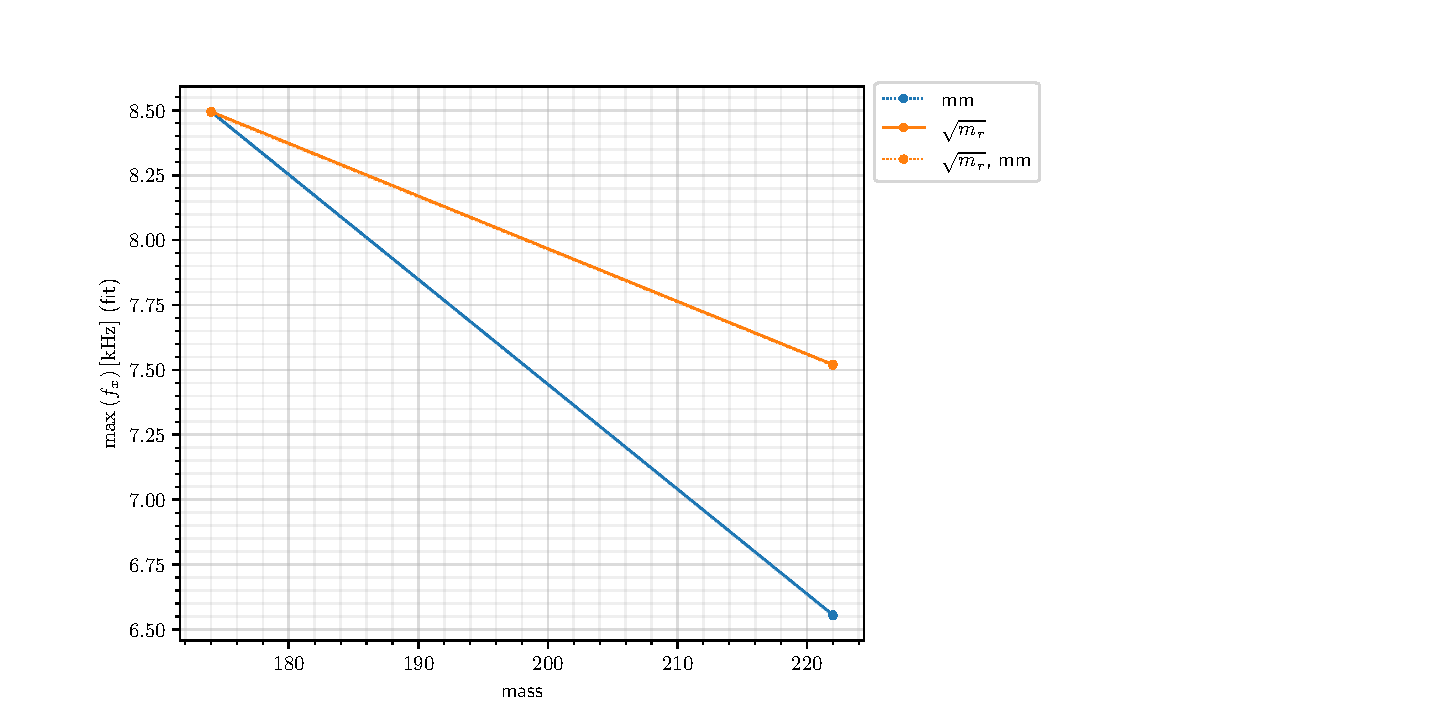
\includegraphics[width=1.2\textwidth]{graphics/micromotion_and_sqrt_freqs_effect.pdf}
	\end{center}
	\caption{The collective $x$-axis movement's frequencies of a 2-species-mixed ion cloud, positioned in a spatial offset from the origin at $t=0$. Dashed v.s solid line-style represents whether \texttt{micromotion} was enabled, and the \texttt{naive\_freqs} parameter is represented in color. The color-varied behavior demonstrates the non-negligible difference between the naive, $\sqrt{m_r}$-based calculation and the real frequencies that are experienced in a real ion trap. Looking closely, you should observe that the dashed lines are right on top of the solid lines - proving that indeed the simulation code was capable of putting the correct forces no matter whether \texttt{micromotion} was enabled or not. The only physically implementable line is the dashed \texttt{mm} labeled line. This figure was generated via fitting\cite{scipy} the cloud's center to a cosine, and via extracting the optimized frequency. Almost identical results can be obtained via using \texttt{numpy.fft.fft}\cite{numpy}.}
	\label{fig:LAMMPS_summarized_naive_freqs-micromotion}
\end{figure}

\section{Coulomb Energy Effect on Temperature}\label{sec:comp/coulomb}

We wish to study sympathetic cooling starting from a thermodynamically stable state. This helps reduce the random effects of thermodynamic instabilities, which can be computationally expensive to ignore, although in experiment, these instabilities might not affect much the cooling. This raises a few important questions: How significant is the Coulomb potential energy in the Boltzmann ensemble? Should it be considered when initiating the positions and velocities of the ions?

Under the secular approximation, and when ignoring the Coulomb potential, the Maxwell-Boltzmann partition function dictates the probability of finding an ion in a position $\mathbf{x}$ to be:

\begin{equation}
	\prod_{i=1}^3 \sqrt{\frac{k_i}{2\pi K_\text{B} T}} \exp\left(\frac{-k_i x_i^2}{2 K_\text{B} T}\right)
	\label{eq:position-probability}
\end{equation}

Where $k_i$ is the spring-like coefficients of the harmonic trap. This distributions couples naturally density and temperature. We are interested in measuring the Coulomb energy per particle (denoted as $E_c/N$) as a function of the parameters of the distribution function above. Since the real temperature is affected by the Coulomb energy, we will not use the symbol $T$ in the following usages of expression \ref{eq:position-probability}, but rather we'll use $\tau$. The parameters that can affect $E_c/N$ are: $\{k_i\}$, $\tau$, and most importantly the number of ions $N$.

The relation of $E_c/N$ to it's parameters is not analytical, yet we still expect a smooth behavior if we'd average over enough randomness. In figure \ref{fig:coulomb_energy} we can see that (expectedly), dense and cold ion clouds produce a higher Coulomb energy, that even exceeds $\tau$.\footnote{Figure \ref{fig:coulomb_energy_normalized} to appendix shows the same results normalized to $\tau$.}

\begin{figure}
	\begin{center}
		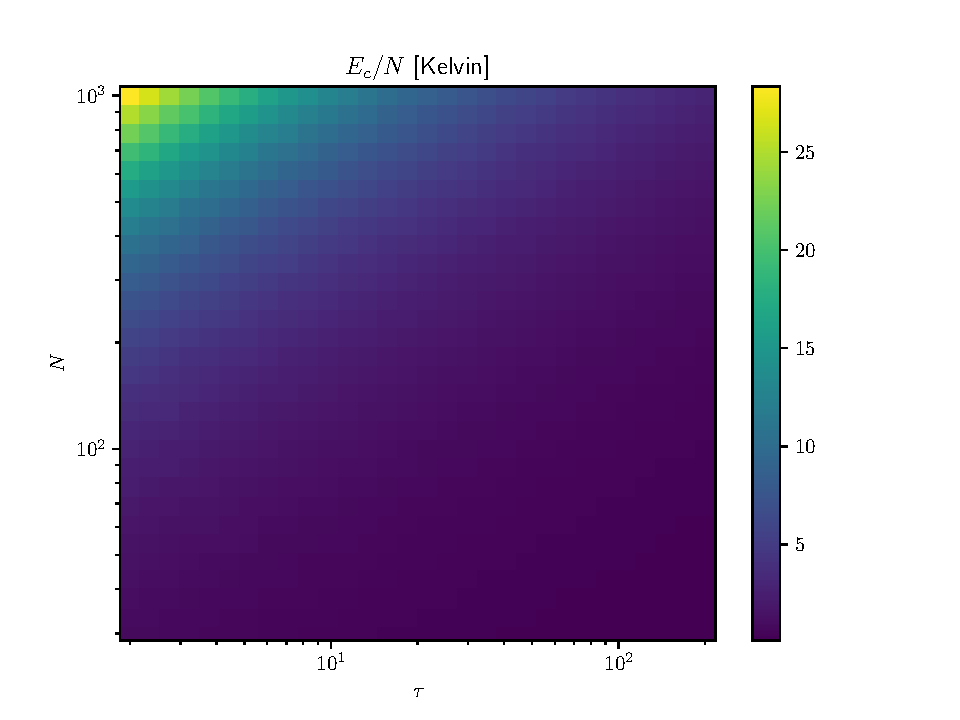
\includegraphics[width=0.95\textwidth]{graphics/coulomb_energy_example@coulomb_energy.pdf}
	\end{center}
	\caption{Example dependence of $E_c/N$ to $N$ and $\tau$ for a trap of \ce{Yb^+} with secular frequencies of $(8.5, 8.5, 1.5) \mathrm{kHz}$, in the range of $\tau\in[2, 200]\mathrm{K}$.}\label{fig:coulomb_energy}
\end{figure}

To produce this color-mesh, we distributed the ions in space multiple times per $(\tau,N)$ point, until the relative standard deviation of all $E_c/N$ results in that point was lower then $0.12$ (arbitrary number), with a minimum of 5 distributions (also termed 'iterations'). Statistical results of figure \ref{fig:coulomb_energy} is depicted in figures \ref{fig:coulomb_energy_std} and \ref{fig:coulomb_energy_iterations}.

Naturally, the value of the highest Coulomb energy found escalates with the trap's tightness, as can be seen in figure \ref{fig:coulomb_energy_f_z}.

\begin{figure}
	\begin{center}
		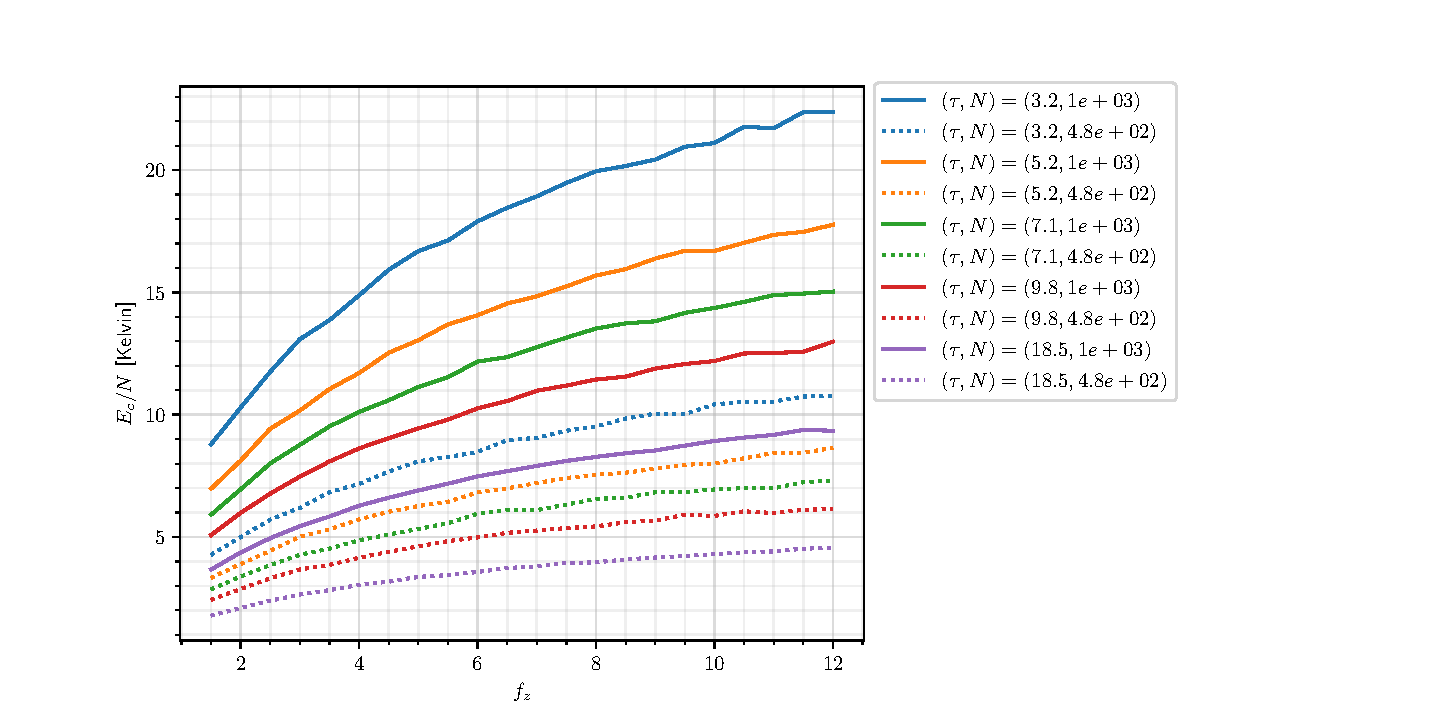
\includegraphics[width=1.2\textwidth]{graphics/coulomb_energy_f_z.pdf}
	\end{center}
	\caption{The dependence of $E_c/N$ upon the z secular frequency, for a few specific $(\tau,N)$ pairs, and $f_x = f_y = 8.5\mathrm{kHz}$.}\label{fig:coulomb_energy_f_z}
\end{figure}

To \textbf{summarize}, the Coulomb energy is not negligible for dense \& cold distributions. Our ability to initiate a distribution of ions in a thermodynamically stable set of positions is limited by the effects of strong Coulomb energy, and by the tightness of our trap. To avoid too strong Coulomb energy effects, we thereby avoid distributing ions in $T < 5\mathrm{K}$.\footnote{During the research period I tried to construct an algorithm that would get a real temperature $T \ne \tau$, $N$ and a set of secular frequencies, and compute a $\tau$ with which the system will be more thermodynamically stable initially. When this algorithm was used for a single ion species it was slightly effective. However when 2 ion species were used, (with different masses and different $\{k_i\}$ - see section \ref{sec:comp/freqs2aq}), accommodating the algorithm for that case has proved to be too complex, and too slow.} More importantly, we expect time dependent temperature measurements to be offset from the initial temperature $T_i$ on the order of magnitude of the Coulomb energy. Since we also wish to start cooling when the system is thermodynamically stable, the Coulomb energy offset requires us to wait for a few $\mathrm{ms}$, before beginning cooling, as can also be seen from the oscillations in figure. % TODO: \ref{fig:} from results

\section{RF division Finesse, Stability \& Convergence}\label{sec:comp/convergence}

% TODO: Cite the convergence statement
An important performance-affecting issue to consider is the finesse of the time division. As explained in subsection \ref{ssec:T_rf_type}, our time must be divided to an integer amount of RF cycles, which is referred to in software as \texttt{rf\_divisor}. To prove that our time division is fine enough, we can run a simulation with the exact same set of parameters, including the initial conditions, and check whether the temperatures graph is changing less and less as \texttt{rf\_divisor} increases.

As a start, we can take a few

% TODO: Explain how RF division is critical.
